\documentclass{article}
\author{Daniel Monjas Migu\'elez 
 		\\ \\ 2 DGIIM Universidad de Granada}
\title{Ejercicios Matemapli Modelos Matem\'aticos}
\usepackage{enumitem}
\usepackage{amsfonts}
\usepackage{amsmath}
\usepackage{mathrsfs}
\usepackage[utf8]{inputenc}
\usepackage[T1]{fontenc}
\usepackage{graphicx}
\usepackage[hidelinks]{hyperref}
\hypersetup{
	colorlinks=true,
	linkcolor=blue,
	filecolor=magenta,
	urlcolor=cyan,
}

\graphicspath{ {images/} }

\begin{document}
\maketitle

\newpage

\textbf{Ejercicio 1:}Dados $\alpha > 0$ y $\beta > 0$, se define la función: 

\begin{equation*}
f(x)= \left\{ \begin{array}{lcc}
             -\alpha x &   si  & x \geq 0 \\
             \\ \beta x &  si & x < 0
             \end{array}
   \right.
\end{equation*}

\textbf{1.}Representa gráficamente la función f para $\alpha = 1.3$ y $\beta = 0.5$ y estudia la evolución de las soluciones de la ecuación en diferencias

\begin{equation*}
x_{n+1} = f(x_n)
\end{equation*}

si la condición inicial es:

\begin{itemize}
\item $x_0 = 0.6$
\item $x_0 = -0.8$
\end{itemize}

\textbf{2.}Determina las condiciones que deben cumplir $\alpha$ y $\beta$ para que p=0 sea un punto de equilibrio asintóciamente estable. \\ \\

\textbf{Apartado 1:}
\begin{figure}[h]
\centering
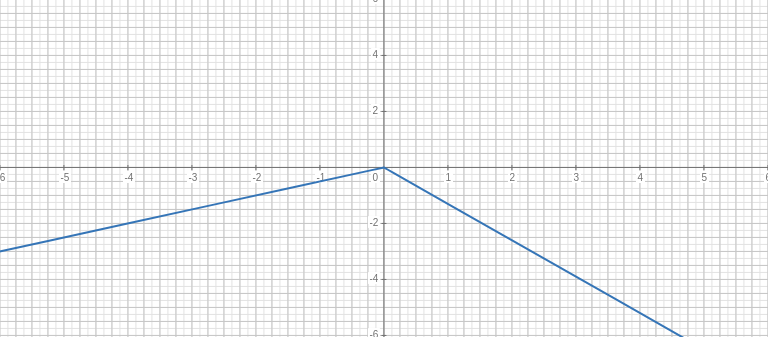
\includegraphics[width=1\textwidth ,scale=1]{funcion_matemapli.png}
\end{figure}

Sea $x_0 = 0.6$, como $x_0 > 0$ se tiene que $x_1 = f(x_0) = -\alpha x$. Definimos la solución general de la ecución en diferencias $x_{n+1} = -\alpha x_n$, cuyo polinomio característico es $P(\lambda)=\lambda + \alpha$ donde $P(\lambda) = 0 \Leftrightarrow \lambda = -\alpha$, luego la solución general sería $x_{n+1} = c_0\cdot(-1.3)^n$, teniendo en cuenta que el dato inicial es $x_0 = 0.6$ se tendría que $c_0 = 0.6$, luego $x_{n+1} = (0.6)\cdot(-1.3)^n$. Esta solución claramente alterna terminos, luego $x_1 < 0$. Por tanto $x_2 = f(x_1) = \beta x_1$, luego definiremos una segunda ecuación en diferencias cuyo valor inicial será $y_0 = -0.78 = 0.6\cdot(-1.3)$. $y_{n+1} = \beta y_n$ donde el polinomio característico asociado es $P(\lambda)= \lambda - \beta$ y se verifica que $P(\lambda) = 0 \Leftrightarrow \lambda = \beta$ y como el dato inicial es $y_0 = x_1 = -0.78$ se tiene que $y_{n+1} = -0.78\cdot(0.5)^n$ que es menor que cero $\forall n \in \mathbb{N}$, luego a partir de $x_1$ se sigue la ecuación en diferencias anterior donde es claro que,

\begin{equation*}
\lim_{n \to \infty} y_n = 0
\end{equation*}

luego como a partir de $x_1$ todos los términos son menores que 0 se verifica las segunda ecuación en diferencias y para el datos $x_0 = 0.6$ las soluciones tienden a 0 por la izquierda. \\ \\

Sea $x_0 = -0.8$, entonces como $x_0 < 0$ tendremos que $x_1 = f(x_0) = \beta x_0$. Definimos la solución de la ecuación en diferencias $x_{n+1} = \beta x_n$, cuyo polinimio característico asociado es $P(\lambda) = \lambda - \beta$ donde $P(\lambda)= 0 \Leftrightarrow \lambda = \beta$ luego como $x_0 = -0.8$ se tiene que la solución general de la ecucación en diferencias para la condición inicial $x_0=-0.8$ es $x_{n+1} = (-0.8)\cdot(0.5)^n$ donde esta solución es claramente menor que 0 $\forall n \in \mathbb{N}$. Luego se sigue esta solución $\forall n \in \mathbb{N}$, que claramente verifica que,

\begin{equation*}
\lim_{n \to \infty} x_n = 0
\end{equation*}

Luego hemos visto que se verifica que para ambas condiciones iniciales que las soluciones tienden a 0. \\ \\

\textbf{Apartado 2:} Claramente es claro que $p=0$ es un punto de equilibrio pues $\alpha \cdot p = 0$ para cualquier $\alpha$.
Usando el apartado anterior vemos que si la condición inicial $x_0$ es un número positivo, sea cual sea, se verificará que $x_1$ es menor que 0, pues por hipótesis $\alpha > 0$, luego $-\alpha < 0$, y por consiguiente $x_0 \cdot -\alpha < 0$. Luego a partir de $x_1$ se utiliza la solución de la ecuación en diferencias $y_{n+1}=x_n \cdot (\beta)^n$, que sabemos que converge a 0 si y sólo si $\beta < 1$, además por hipótesis tenemos que $\beta > 0$. Si la condición inicial fuese negativa se trabaja directamente con la solución general de $x_{n+1}=x_n \cdot \beta$, que converge a 0 si y sólo si $\beta < 1$. Luego si $\alpha \in \mathbb{R}+$ y $0 < \beta < 1$, para cualquier punto de un entorno de 0 se verificará que al aplicar $x_{n+1} = f(x_n)$ $\lim_{n \to \infty} x_n = 0$, luego si $\alpha \in \mathbb{R}^+$ y $0 < \beta < 1$ el punto p=0 será asintóticamente estable. \\ \\

\textbf{Ejercicio 2:} Dado $\alpha > 0$, se considera la ecuación en diferencias:
\begin{equation*}
x_{n+1} = 1 - \alpha|x_n|
\end{equation*}

\begin{enumerate}
\item Para $\alpha = 0.4$, estudia gráficamente el comportamiento de las soluciones en función de su dato inicial $x_0 \in \mathbb{R}$.
\item Para $\alpha > 0$ determina el número de puntos de equilibrio de la ecuación en diferencias.
\item Estudia la estabilidad de los puntos de equilibrio para $\alpha = 1.3$.
\item Si $\alpha = 2$, comprueba que $\{-0.2,0.6\}$ es un 2-ciclo y estudia su estabilidad.
\end{enumerate}

\textbf{Solución:} Primero para facilitar el trabajo posterior defino $f(x) = 1 - \alpha|x|$ y desdoblamos lo anterior en una función por partes de la siguiente manera,

\begin{equation*}
f(x)= \left\{ \begin{array}{lcc}
             1 -\alpha x &   si  & x \geq 0 \\
             \\ 1 + \alpha x &  si & x < 0
             \end{array}
   \right.
\end{equation*}
\textbf{Apartado 1:} \\ \\
\textbf{Apartado 2:}Para realizar el estudio de los puntos de equilibrio estudiaremos dos casos:

\begin{itemize}
\item $x = 1 - \alpha x$, donde despejando la ecuación anterior se llega a $x = \frac{1}{1+\alpha}$. Como $\alpha > 0$ claramente $1 + \alpha > 0$ y por consiguiente $\frac{1}{1+\alpha}$, luego $p = \frac{1}{1 + \alpha}$ es un punto de equilibrio, para todo $\alpha > 0$.

\item $x = 1 + \alpha x$, donde despejando la ecuación anterior se llega a $x = \frac{1}{1 - \alpha}$. Para que el punto anterior sea de equilibrio se tiene que verificar que $\frac{1}{1 - \alpha} < 0$ luego se deberá verificar que $1 - \alpha < 0 \Rightarrow \alpha > 1$.
\end{itemize}

En conclusión, la función tendrá dos puntos de equilibrio si $\alpha > 1$, en caso contrario sólo tendra un punto de equilibrio. \\ \\

\textbf{Apartado 3:} Usando el apartado anterio como $\alpha > 1$ se tendran dos puntos de equilibrio, $p_1 = \frac{1}{1 + \alpha} = \frac{1}{2.3} \approx 0.43478$. Claramente la función f(x) es continua en el punto $p_1$ luego calcularemos la derivada.

\begin{equation*}
f'(x)= \left\{ \begin{array}{lcc}
             -1.3 &   si  & x \geq 0 \\
             \\ 1.3 &  si & x < 0
             \end{array}
   \right.
\end{equation*}

utilizando esta derivada vemos que $f'(p_1) \notin (-1,1)$, luego el punto de equilibrio $p_1$ no es asintóticamente estable. \\

Calculamos ahora $p_2 = \frac{1}{1-1.3}= \frac{1}{-0.3} \approx -3.33$ utilizando la derivada calculada para el caso anterior se tiene que $f'(p_2) \notin (-1,1)$, luego el punto de equilibrio $p_2$ tampoco es asintóticamente estable. Luego para $\alpha = 1.3$ ninguno de los puntos de equilibrio de la función es asintóticamente estable. \\ \\

\textbf{Apartado 4:} Probaremos que es un dos ciclo, luego $f(-0.2) = 1 + 2\cdot(-0.2) = 0.6$ y $f(0.6)= 1 - 2\cdot0.6 = -0.2$, luego queda demostrado que $\{-0.2,0.6\}$ es un 2-ciclo. Para ver que sea asintóticamente estable usaremos la regla de la cadena. Llamaremos $g(x) = 1 - \alpha x$ y $h(x) = 1 + \alpha x$. Luego,

\begin{equation*}
(g \circ h)'(-0.2) = g'(h(-0.2))\cdot h'(-0.2) = g'(0.6) \cdot 2 = -2 \cdot 2 = -4 \notin (-1,1)
\end{equation*}

si se compone $h \circ g$ al aplicar la regla de la cadena se ve a simple vista que $(h \circ g)'(0.6) = -4 \notin (-1,1)$ luego el 2-ciclo es claramente inestable. \\ \\

\textbf{Ejercicio 3:} Una determinada población está estructurada en base a tres grupos diferentes de edad: crías (hasta los 3 años), jóvenes (de 3 a 6 años) y adultos (de 6 a 9 años). Es conocido que las crías no engendran nuevas crías, que cada joven engendra en media 1 cría y cada adulto engendra en media 8 crías. Además, las observaciones arrojan el dato de que la mitad de las crías llegan a jóvenes, en tanto que sólo el 51.1\% de los jóvenes sobrevive.

\begin{enumerate}
\item Escribe el sistema de ecuaciones en diferencias que describe la evolución de la población así como su formulación matricial. ¿Es la matriz del sistema una matriz de Leslie?¿Es egódica?.

\item Representa el grafo asociado a dicha matriz. ¿Es la matriz irreducible?

\item Si la población inicial consiste en 10 crías, 8 jóvenes y 12 adultos, ¿cuál será la distribución de la población al cabo de 9 años?

\item ¿Podemos asegurar que la matriz tiene un valor propio dominante? Justifica tu respuesta.

\item Estudia la evolución de la población a largo plazo, indicando la distribución de su priámide de edad.

\item Utilizando las ecuaciones descritas en el primer apartado y mediante sustituciones sucesivas, determina una ecuación en diferencias de orden 3 para el número de crías. ¿Qué relación existe entre el polinomio característico de esta ecuación y el de la matriz del apartado 1?¿Tiene la ecuación un punto de equilibrio?¿Es asintóticamente estable?

\item Resuelva la ecuación y comprueba que se obtienen los mismo resultados que en los apartados 3 y 5.
\end{enumerate}

\textbf{Solución:} \\
\textbf{Apartado 1:}
En primer lugar definiremos los tres estadios posibles de los que dispone la población:

\begin{itemize}
\item $c_n$=crías en el periodo n
\item $j_n$=jóvenes en el periodo n
\item $a_n$=adultos en el periodo n
\end{itemize}

, en el enunciado se nos proporciona la siguiente información,

\begin{itemize}
\item $f_c = 0$ donde $f_c$ es la tasa de fertilidad de las crías.
\item $f_j = 1$ donde $f_j$ es la tasa de fertilidad de los jóvenes.
\item $f_a = 8$ donde $f_a$ es la tasa de fertilidad de los adultos.
\item $s_c = 0.5$ donde $s_c$ es la tasa de supervivencia de las crías.
\item $s_j = 0.511$ donde $s_j$ es la tasa de supervivencia de los jóvenes.
\item $s_a = 0$ donde $s_a$ es la tasa de supervivencia de los adultos.
\end{itemize}

, a partir de los datos anteriores podemos definir el siguiente sistema de ecuaciones en diferencias,

\begin{equation*}
\left\{ \begin{array}{lcc}
             c_{n+1} = j_n + 8\cdot a_n \\
             \\ j_{n+1} = 0.5\cdot c_n \\
             \\ a_{n+1} = 0.511\cdot j_n
             \end{array}
   \right.
\end{equation*}

, cuya matriz asociada es la siguiente,

\begin{equation}
\begin{pmatrix}
c_{n+1} \\
j_{n+1} \\
a_{n+1}
\end{pmatrix} 
=
\begin{pmatrix}
0 & 1 & 8 \\
0.5 & 0 & 0 \\
0 & 0.511 & 0
\end{pmatrix}
\cdot
\begin{pmatrix}
c_n \\
j_n \\
a_n 
\end{pmatrix}
\end{equation}

Verifica que todos los miembros de la primera fila son mayores o iguales que cero, y a partir de la segunda fila todo son ceros menos la posición [fila][fila-1] que contiene un coeficiente $s_i$ con $0 < s_i \leq 1$, luego es una matriz de Leslie. \\

Sabiendo que una matriz es ergódica si ella misma o alguna potencia suya tiene todos sus coeficientes positivos. Claramente la expresión matricial obtenida no tiene todos sus coeficientes postivos, luego calcularemos sus potencias, llegando a,

\begin{equation*}
\begin{pmatrix}
0 & 1 & 8 \\
0.5 & 0 & 0 \\
0 & 0.511 & 0
\end{pmatrix}
^5 = 
\begin{pmatrix}
2.044 & 8.6059 & 2 \\
0.125 & 2.044 & 8.176 \\
0.52224 & 0.12775 & 1.022
\end{pmatrix}
\end{equation*}

, cuyos coeficientes son todos postivos luego las matriz es ergódica. \\ 

\textbf{Apartado 2:}
Una matriz se considera irreducible si su digrafo o grafo dirigido es fuertemente conexo, es decir, si se puede encontrar un camino de ida y uno de vuelta para cada par de nodos i, j con $i \neq j$. Si nos fijamos en el grafo obtenido, tenemos

\begin{itemize}
\item 1->2, por medio de la arista que los une
\item 1->3, pasando por dos.
\item 2->3, por medio de la arista que los une
\item 2->1, por medio de la arista que los une
\item 3->1, por medio de la arista que los une
\item 3->2, pasando por 1.
\end{itemize}

Luego viendo este análisis tenemos que el grafo obtenido es fuertemenete conexo y por tanto la matriz es irreducible.
\begin{figure}[t]
\centering
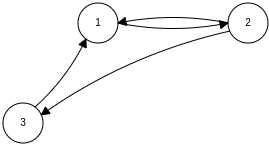
\includegraphics[width=0.7\textwidth,scale=1]{grafo_dirigido.png}

\end{figure}
\\ \\

\textbf{Apartado 3:}
El ejercicio pregunta por cuál será la distribución de la población al cabo de 9 años. Como en este modelo cada estadío requiere de tres años, entonces se pide la distribución de individuos tras transcurrir 3 estadíos, es decir, $c_3$, $j_3$ y $a_3$, con distribución de tamaños inicial $L=(10,8,12)^T$. Que será el número de individuas en cada estadío para al transcurrir 9 años. Luego llamando A a la expresión matricial obtenida en el apartado 1 realizamos la siguiente operación.

\begin{equation}
A^3 \cdot L =
\begin{pmatrix}
2.044 & 0.5 & 4 \\
0.25 & 2.044 & 0 \\
0 & 0.2555 & 2.044
\end{pmatrix}
\cdot 
\begin{pmatrix}
10 \\
8 \\
12 
\end{pmatrix}
=
\begin{pmatrix}
72.44 \\
18.852 \\
26.572 \\
\end{pmatrix}
\end{equation}

, redondeando obtenemos 72 crías, 19 jóvenes y 27 adultos. Luego la distribución sería 61.02\% crías, 16.1\% jóvenes y 22.88\% adultos, tras nueve años. \\ \\

\textbf{Apartado 4:} Si el producto de dos elementos consecutivos de la primera fila de una matriz de Leslie es estrictamente positivo, podemos asegurar que tiene un único valor propio real y positivo que es simple y dominante. En la primera fila de la matriz de Leslie obtenida en el apartado uno encontramos, consecutivamente, los coeficientes 1 y 8, cuyo producto es estrictamente positivo, luego podemos asegurar que esta tendrá un único valor propio real y positivo que es simple y dominante. \\ \\

\textbf{Apartado 5:} En primer lugar calcularemos cual es el valor propio dominante que por el apartado anterior sabemos que es real y positivo (llamaremos A a la matriz de Leslie del apartado 1).

\begin{equation*}
det(A - \lambda I)=det(
\begin{pmatrix}
-\lambda & 1 & 8 \\
0.5 & -\lambda & 0 \\
0 & 0.511 & -\lambda
\end{pmatrix}
)=-\lambda^3+0.5\lambda+2.044
\end{equation*}

, al igualar a 0 y resolver la ecuación obtenemos los valores propios,

\begin{equation*}
-\lambda^3+0.5\lambda+2.044 = 0 \Leftrightarrow \lambda = \frac{7}{5} \> ó \> \lambda = -\frac{7}{10}+i\frac{\sqrt{97}}{10} \> ó \> \lambda = -\frac{7}{10}-i\frac{\sqrt{97}}{10}
\end{equation*}

,luego llegamos a que el valor propio dominante es $\lambda = \frac{7}{5}$. A partir de este valor propio calculamos el subespacio asociado al mismo y el vector generador de este y lo normalizamos.

\begin{equation*}
V_{\frac{7}{5}}=\{(x,y,z)\in \mathbb{R}^3 : 
\begin{pmatrix}
-\frac{7}{5} & 1 & 8 \\
0.5 & -\frac{7}{5} & 0 \\
0 & 0.511 & -\frac{7}{5}
\end{pmatrix}
\cdot
\begin{pmatrix}
x \\
y \\
z 
\end{pmatrix}
=
\begin{pmatrix}
0 \\
0 \\ 
0
\end{pmatrix}
\}
\end{equation*}

la última fila de la matriz anterior es combinación lineal de la primera y la segunda, luego se puede suprimir llegando a lo siguiente,

\begin{equation*}
V_{\frac{7}{5}}=\{(x,y,z)\in \mathbb{R}^3: \left\{ \begin{array}{lcc}
             -\frac{7}{5}x+y+8z=0\\
             \\ \frac{1}{2}x-\frac{7}{5}y = 0
             \end{array}
   \right. \}
\end{equation*}
, como se disponen de dos ecuaciones y tres incógnitas se trata de un subespacio de dimensión uno, luego será generado por un vector cuyas coordenadas satisfagan las ecuaciones. Luego una vez más podemos reescribir como,

\begin{equation*}
V_{\frac{7}{5}}=L(\{(560,200,73)\})
\end{equation*}

, donde L hace referencia a combinación lineal. Luego $(560,200,73)$ sería una vector propio asociado al valor propio $\lambda =\frac{7}{5}$. Ahora normalizamos este vector usando la norma 1. Obteniendo $v'=(\frac{560}{833},\frac{200}{833},\frac{73}{833}) \approx (0.6723,0.2401,0.0876)$, luego a largo plazo la distribución sería 67.23\%, jóvenes 24.01\% y adultos 8.76\%. Además como el valor propio dominante de esta matriz es mayor que 1 se verifica que la población crece indefinidamente. \\

Por último se inserta una imagen de la pirámide de edad (\ref{pirámide}). 
\begin{figure}[h]
\caption{Piramide de Edad Apartado 5}
\label{pirámide}
\centering
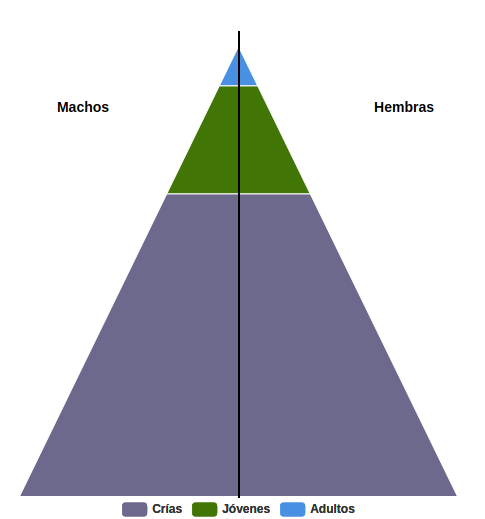
\includegraphics[width=0.8\textwidth, scale=1]{piramide.png}
\end{figure}
\\ \\

\textbf{Apartado 6:}Despejando el sistema de ecuaciones del primer apartado tenemos que,

\begin{equation*}
\left\{ \begin{array}{lcc}
             c_{n+1} = j_n + 8\cdot a_n \\
             \\ j_{n+1} = 0.5\cdot c_n \Rightarrow j_n = 0.5c_{n-1} \\
             \\ a_{n+1} = 0.511\cdot j_n = 0.2555\cdot c_{n-1} \Rightarrow a_n = 0.2555\cdot c_{n-2}
             \end{array}
   \right.
\end{equation*}

, sustituyendo en la primera de las ecuaciones tenemos que,

\begin{equation*}
c_{n+1}=0.5\cdot c_{n-1} + 2.044\cdot c_{n-2}
\end{equation*}

, que sería una ecuación de orden 3 para el número de crías. \\

Ahora definimos su polinomio característico $P(\lambda)=\lambda^3-0.5\lambda - 2.044$, que es el polinomio caraterístico de la matriz multiplicado por -1, luego tenemos que las soluciones son las mismas. \\

Ahora buscamos un punto de equilibrio para esa ecuación en diferencias.

\begin{equation*}
x_*-0.5x_*-2.044x_* = 0
\end{equation*}
, donde obtenemos el punto fijo x=0. Este punto fijo no puede ser estable, pues hemos visto que el valor dominante de la matriz de Leslie es mayor que 1, por consiguiente la población crecerá ilimitadamente. Como esta ecuación en diferencias estudia el comportamiento de las crías y la población crece ilimitadamente, es claro que p=0 no puede ser asintóticamente estable, pues si lo fuese la población no crecería ilimitadamente. \\ \\

\textbf{Apartado 7:} Como ya comentamos en el apartado anterior el polinomio característico asociado a la ecuación en diferencias es el mismo que el de la matriz de Leslie multiplicado por menos uno, luego conocemos ya las raíces del mismo. A partir de aquí calcularemos el módulo y el ángulo para las raíces complejas,

\begin{equation*}
|\lambda_1|=|\lambda_2| = \sqrt{(\frac{7}{10})^2 + (\frac{\sqrt{97}}{10})^2}=\frac{\sqrt{146}}{10}
\end{equation*}

, una vez calculado el módulo, que es el mismo para las dos raíces complejas procedo a calcular el ángulo,

\begin{equation*}
\theta = arctan(\frac{\sqrt{97}/10}{-7/10})=arctan(\frac{\sqrt{97}}{-7}) \approx 1.697\pi
\end{equation*}

con esto defino la solución general,

\begin{equation*}
x_{n+1} = k_0\cdot(\frac{7}{5})^n + (\frac{\sqrt{146}}{10})^n\cdot(k_1\cdot cos(n\theta) + k_2\cdot sen(n\theta))
\end{equation*}

conocidos $c_0$, $j_0$ y $a_0$, gracias al enunciado del apartado 3, procedemos a calcular $c_1$ y $c_2$ utilizando el sistema de ecuaciones en diferencias del apartado 1 y los resultados obtenidos en el apartado 5, llegando a,

\begin{itemize}
\item $c_0 = 10$
\item $c_1 = 8 + 12\cdot8=104$
\item $c_3 = 0.5\cdot c_1 + 2.044\cdot c_1 = 72.44$
\end{itemize}

con esto resolvemos el siguiente sistema de ecuaciones,

\begin{equation*}
\left\{ \begin{array}{lcc}
             k_0 + k_1 = 10 \\
             \\ \frac{7}{5}\cdot k_0 + \frac{\sqrt{146}}{10}\cdot cos(\theta) k_1 + \frac{\sqrt{146}}{10}\cdot sen(\theta) k_2 = 104 \\
             \\ \frac{343}{125} \cdot k_0 + \frac{146\cdot\sqrt{146}}{1000}\cdot cos(3\cdot \theta) k_1 + \frac{146}{100}\cdot cos(3\cdot \theta) k_1 = 72.44
             \end{array}
   \right.
\end{equation*}

,tras resolver el sistema de ecuaciones podemos reescribir la solución general como,

\begin{equation*}
x_{n+1} = 10\cdot(\frac{7}{5})^n + (\frac{\sqrt{146}}{10})^n\cdot(0.00035457 \cdot cos(n\theta) -91.381\cdot sen(n\theta))
\end{equation*}

vamos ahora que se verifican los apartados 3 y 5.

Claramente esta ecuación verifica el apartado 3, pues se han tomado los coeficientes de forma que lo cumple. Veamos ahora que también verifica el apartado 5. Viendo que $\frac{7}{5} > 1$, que $\frac{7}{5} > \frac{\sqrt{146}}{10}$ y que el creciemiento de $\frac{\sqrt{146}}{10}^n$ es más lento que el de $\frac{7}{5}^n$, se tendrá que:

\begin{equation*}
\lim_{n \to \infty} c_n = \infty
\end{equation*}

luego como ya habíamos dicho en apartados anteriores la población crece ilimitadamente.
\end{document}